\section{Theorie}
\label{sec:Theorie}

Wenn ein Photon auf ein freies Elektron trifft, wird das Photon gestreut.
Dieser Prozess wird Compton-Streuung genannt.
Dabei gibt das Photon ein Teil seiner Energie an das Elektron ab wodruch sich die Wellenlänge des Photons zu einer höheren Wellenlänge hin verschiebt.
Die Wellenlängenverschiebung lässt sich dabei gemäß der Gleichung 
\begin{equation}
    \Delta \lambda = \lambda _\text{C}(1-cos(\theta))
    \label{eq:verschiebung}
\end{equation}
berechnen.
Dabei entspricht $\Delta \lambda$ der Differenz der eingehenden Wellenlänge des Photons und der ausgehenden Wellenlänge des Photons.
Der Winkel $\theta$ ist der Winkel in dem das Photon zu seiner ursprünglichen Bahn gestreut wird.
Der Prozess ist schematisch in der Abbildung \ref{fig:streuung} zu erkennen.
\begin{figure}
    \centering
    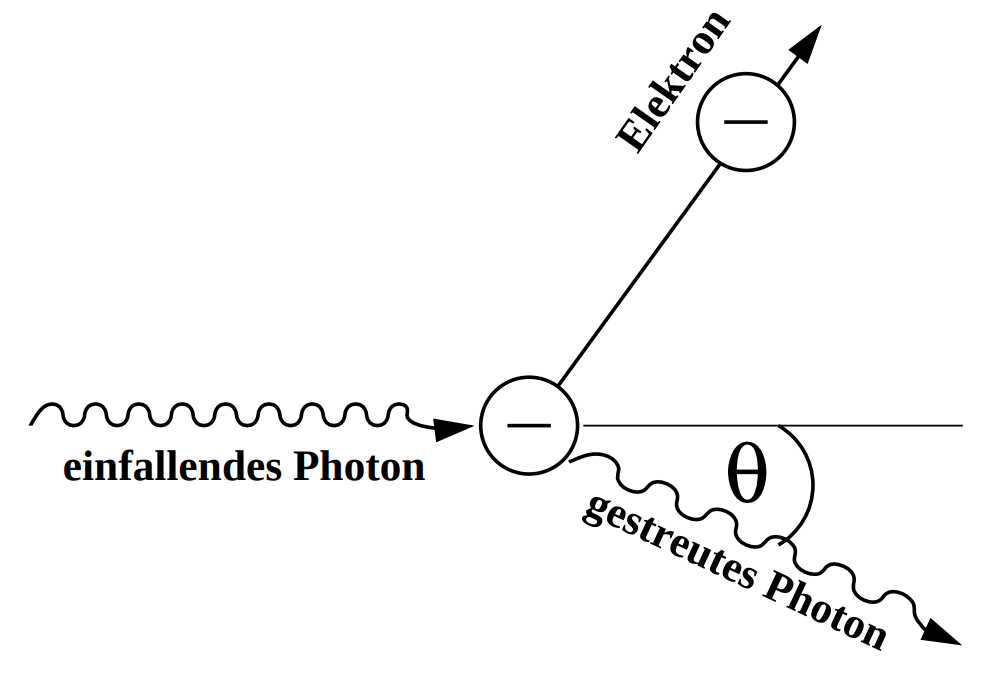
\includegraphics[width=\textwidth/2]{content/data/streuung.png}
    \caption{Eine schematische Darstellung der Streuung eines Photons am Elektron durch den Comptoneffekt, entnommen aus \cite{anleitung}}
    \label{fig:streuung}
\end{figure}
Wie an der Gleichung \eqref{eq:verschiebung} unschwer zu erkennen ist, wird die Wellenlänge des Phtotons am stärksten verringert, wenn dieses mit einem Winkel von $\theta = 180 \si{\degree}$ gestreut wird.
An diesem Punkt ist $\Delta \lambda = 2 \lambda _\text{C}$.
\\\\
Für die Erzeugung von Photonen wird eine Röntgenröhre genutzt.
Diese erzeugt Elektronen an einer Glühkathode.
Nach dem austreten aus der Kathode, werden die Elektronen, durch das starke elektrische Feld zwischen Kathode und Anode in Richtung Anode beschleunigt.
Beim Auftreffen auf der Anode entsteht nun die Röntgenstrahlung.
Diese setzt sich aus einem kontinuierlichem Bremsspektrum und der charakteristischen Strahlung des Anoden Materials zusammen.


Um die Wellenlänge der Strahlung zu bestimmen wird die Bragg'sche Reflexion an einem LiF-Krsitall beziehungsweise eines Plexiglas-Streuer genutzt.
Die Strahlung, die auf den Kristall trifft wird von diesem reflektiert.
Dabei ist zu beachten, dass ein Kristall ein dreidimensionales Gitter bildet.
Der Krsitall reflektiert also nicht nur an seiner obersten Ebene die Strahlung sondern auch in den unteren Gitterschichten.
Die verschieden reflektierten Röntgenstrahlen, interferieren nach der Reflexion miteinander.
So kann die Wellenlänge der reflektierten Strahlung nach Beugung erster Ordnung durch die Gleichung
\begin{equation}
    2 d \sin(\alpha) = \lambda
    \label{eq:bragg}
\end{equation}
berechnet werden.
$\alpha$ ist hier der Winkel in dem der Krsitall zur Strahlung steht und $d$ der Gitterabstand des Kristalls.

Zur Messung der Intensität der Strahlung wird ein Geiger-Müller-Zählrohr genutzt.
Dieses misst die einkommenden Impulse pro Sekunde.
Allerdings muss eine Totzeit $\tau$ eingerechnet werden um aus den Impulsen die Intensität errechnen zu können.
Wenn die Totzeit bekannt ist kann durch 
\begin{equation}
    I = \frac{N}{1-\tau N}
    \label{eq:intens}
\end{equation}
die Intensität berechnet werden.
